\section{Processi organizzativi}
	\subsection{Gestione progetto}
	\subsubsection{Scopo}
	Lo scopo di questo processo è quello di fornire al gruppo delle linee guida su come gestire l'organizzazione delle varie fasi del progetto, con i punti a seguito elencati:
	\begin{itemize}
		\item Gestione dei ruoli;
		\item Gestione delle comunicazioni;
		\item Gestione degli incontri;
		\item Gestione per il controllo della versione;
		\item Gestione del GitHub Workflow\textsubscript{G};
		\item Gestione del tracciamento delle attività.
	\end{itemize}
	\subsubsection{Gestione ruoli}
	Durante il corso del progetto il gruppo dovrà gestire i vari ruoli garantendo una suddivisione equa tra i membri e pertinente rispetto al processo in svolgimento.\\
	I sei ruoli possibili da assegnare sono:
    \begin{itemize}
    	\item Responsabile;
    	\item Amministratore;
    	\item Analista;
    	\item Progettista;
    	\item Programmatore;
    	\item Verificatore.
    \end{itemize}
	\subsubsubsection{Responsabile}
	Il responsabile di progetto è la figura di riferimento con l'esterno, quindi  garantisce una buona comunicazione con proponente e committente. Si assume inoltre la responsabilità delle scelte del gruppo, dopo averle approvate.\\
	Il responsabile quindi gestisce:
	\begin{itemize}
		\item Elaborazione di piani e scadenze del progetto;
		\item Gestire la suddivisione dei ruoli all'interno del gruppo;
		\item Approvare il rilascio di prodotti parziali o finali, come documentazione o software;
		\item Analisi e gestione dei rischi.
	\end{itemize}
	\subsubsubsection{Amministratore}
	L'amministratore di progetto ha lo scopo di controllare l'efficienza dell'ambiente di lavoro, assicurandosi quindi che gli strumenti di supporto alle norme di progetto siano usati correttamente da tutti i membri del gruppo.\\
	L'amministratore quindi gestisce:
	\begin{itemize}
		\item La corretta applicazione delle norme di progetto;
		\item La ricerca di nuovi metodi per rendere più efficiente l'ambiente di lavoro;
		\item Le versioni dei vari prodotti durante il corso del progetto;
		\item L'analisi di metodi per la gestione della qualità.
	\end{itemize}
	\subsubsubsection{Analista}
	L'analista si occupa di analizzare a fondo il problema e di individuare i vari requisiti\textsubscript{G} che dovrà avere il prodotto finale in base a ciò che si ricava dal capitolato e dai successivi incontri con il proponente. \\
	L'analista quindi gestisce:
	\begin{itemize}
		\item Lo studio approfondito del dominio\textsubscript{G} del problema;
		\item Il documento \textit{Analisi dei requisiti\textsubscript{G}};
		\item L'individuazione dei requisiti\textsubscript{G} del prodotto finale;
		\item L'analisi dei casi d'uso\textsubscript{G}.
	\end{itemize}
	\subsubsubsection{Progettista}
	Il progettista si occupa di trovare soluzioni tecniche e tecnologiche che possano permettere al gruppo di creare un prodotto che rispetti al meglio tutti i requisiti\textsubscript{G} individuati dagli analisti. \\
	Il progettista quindi gestisce:
	\begin{itemize}
		\item La scelta degli aspetti tecnici e tecnologici per la realizzazione del prodotto;
		\item La scelta dei vari modelli da utilizzare nella definizione dell'architettura del prodotto;
		\item Di definire l'architettura del prodotto che verrà poi programmato.
	\end{itemize}
	\subsubsubsection{Programmatore}
	Il programmatore si occupa di codificare le soluzioni individuate dai progettisti per la creazione del prodotto finale. \\
	Il programmatore quindi gestisce:
	\begin{itemize}
		\item La scrittura del codice in modo che sia chiaro e facile da mantenere;
		\item Gli strumenti che si occupano dei test utilizzati per la verifica\textsubscript{G} e la validazione\textsubscript{G} del software;
		\item La redazione del Manuale Utente relativo alla codifica del prodotto.
	\end{itemize}
	\subsubsubsection{Verificatore}
	Il verificatore si occupa di tutte le operazioni di verifica\textsubscript{G} e validazione\textsubscript{G} dei vari prodotti parziali e finali del progetto. \\
	Il verificatore quindi gestisce:
	\begin{itemize}
		\item La verifica\textsubscript{G} e validazione\textsubscript{G} dei prodotti parziali o finali in fase di revisione in modo che rispettino gli obiettivi di qualità imposti nel documento \textit{Piano\_di\_qualifica v 1.0.0}. I seguenti prodotti se a norma verranno di conseguenza integrati;
		\item Segnalare gli eventuali errori riscontrati.
	\end{itemize}
    \subsubsection{Gestione delle comunicazioni}
        \subsubsubsection{Comunicazioni interne}
        Le comunicazioni interne:
        \begin{itemize}
            \item Riguardano solamente i componenti del team;
            \item Avvengono su \textit{WhatsApp};
            \item Utilizzate per:
                \begin{itemize}
                    \item Comunicazioni istantanee tra tutti i componenti;
                    \item Discussioni;
                    \item Pianificazione degli incontri;
                    \item \textit{daily scrum\textsubscript{G} meeting}.
                \end{itemize}
        \end{itemize}
            
        \subsubsubsection{Comunicazioni esterne}
        Le comunicazioni esterne:
        \begin{itemize}
            \item Riguardano il gruppo e le altre figure (proponente e committente);
            \item Utilizzo del dominio\textsubscript{G} di gruppo (\textit{catchemallswe3@gmail.com}) di posta elettronica;
            \item Utilizzate per comunicazioni ufficiali tra il team e le altre figure.
        \end{itemize}

        
        
    \subsubsection{Gestione degli incontri}
        \subsubsubsection{Incontri interni}
        Gli incontri interni sono necessari sia per una corretta adozione del \textit{framework Scrum\textsubscript{G}} (incontro organizzativo settimanale)
        sia per permettere al team di interagire direttamente, discutendo, proponendo e valutando idee, problematiche e possibili 
        soluzioni: per questo si tratta di uno strumento largamente utilizzato
        \newline
        Si predilige la modalità virtuale per comodità cercando di schedulare riunioni in cui tutti riescano a partecipare.
        \newline
        La piattaforma utilizzata è \textit{discord}, la quale permette la creazione e l'utilizzo di:
        \begin{itemize}
            \item Canali testuali;
            \item Canali video (con possibilità di condivisione schermo).
        \end{itemize}
        Al termine degli incontri il responsabile di progetto inserisce nello sprint\textsubscript{G} corrente il compito di redigere i verbali. 

        \subsubsubsection{Incontri esterni}
        Gli incontri esterni sono schedulati in seguito alla presenza di dubbi (implementativi, riguardanti requisiti\textsubscript{G} o richieste di altro tipo) all'interno del 
        team: questi incontri sono preceduti dallo svolgimento di una o più riunioni interne nelle quali si affrontano e si definiscono tali problematiche.
        \newline
        Per quanto riguarda l'organizzazione viene contattato tramite email il referente di progetto proponendogli diverse date e orari affinchè si trovi quella 
        più comoda per entrambe le parti. 
        \newline
        Come per quelli interni gli incontri esterni sono tenuti in modalità virtuale ma a loro differenza si utilizza una riunione \textit{Zoom} definita dal gruppo. 
        \newline
        I verbali hanno lo scopo di documentare in maniera dettagliata tutti gli argomenti trattati affinchè si possa costruire uno storico identificando
        e motivando le decisioni prese.
        \newline
        Come per quelli interni il responsabile di progetto inserisce nello sprint\textsubscript{G} corrente il compito di redigere tali documenti.

	\subsubsection{Versionamento}
	GitHub\textsubscript{G} è lo strumento utilizzato dal gruppo per il versionamento del codice.
	\newline Il team è identificato in tale piattaforma come organizzazione (\href{https://github.com/catchEmAll-SWE}{vedi}).
	Inoltre, al fine di documentare il più possibile, ogni commit\textsubscript{G} che porta valore al progetto contiene il riferimento al ticket che completa (totalmente o anche solo parzialmente). 

	\subsubsection{GitHub Workflow\textsubscript{G}}
	Tutti i titoli e le descrizioni dei commit\textsubscript{G} devono essere fatti in inglese per conformità tra essi.
	\newline Il Workflow viene gestito concorrentemente da GitHub\textsubscript{G} e JIRA\textsubscript{G}. \\
In JIRA\textsubscript{G} vengono create ed organizzate le issue\textsubscript{G}, una volta fatto ciò si procede attraverso github\textsubscript{G} alla creazione del branch\textsubscript{G} relativo alla issue\textsubscript{G} da risolvere.\\
	Tale ramo ha nome codificato come:
	\begin{lstlisting}
		CEA-num-titolo-della-issue\textsubscript{G}
	\end{lstlisting}
	Questo permette di identificare titolo e numero della issue\textsubscript{G} di appartenenza. Una volta fatto ciò viene creato un \textbf{primo commit\textsubscript{G}}, nel cui messaggio è specificata l'avvenuta presa in carico della issue\textsubscript{G}, la quale dovrà passare dallo stato "to do" allo stato "in progress"\\
	Ciò è garantito dal suddetto commit\textsubscript{G} message contenente la stringa:
	\begin{lstlisting}
		CEA-num #open <testo aggiuntivo>
	\end{lstlisting}
	Una volta fatto ciò è possibile lavorare liberamente sul proprio ramo di feature\textsubscript{G}.
	\newline \textbf{Ad ogni} aggiornamento dell'attività svolta si dovrà fare riferimento alla issue\textsubscript{G} e specificare il tempo impiegato per lo svolgimento di tale attività includendo nella descrizione:
	\begin{itemize}
		\item Visual Studio Code;
		\begin{figure}[ht!]
			\centering
			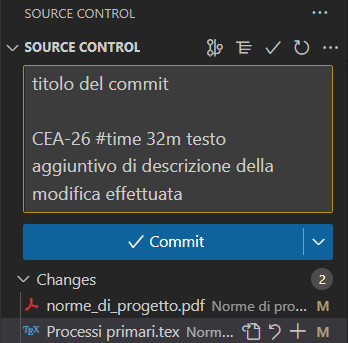
\includegraphics[scale=0.7]{img/visual_code_example.png}
			\caption{Immagine di come scrivere un commit\textsubscript{G} su Visual Studio Code}
		\end{figure}
		\item Git Bash.
		\begin{lstlisting}
	git commit -m "titolo del commit\textsubscript{G}" -m "CEA-26 #time 32m ..."
		\end{lstlisting}
	\end{itemize}
	Comando generico da aggiungere nel corpo del messaggio, non nel titolo del commit\textsubscript{G}:
	\begin{lstlisting}
		CEA-num #time ww dd hh mm <testo aggiuntivo>
	\end{lstlisting}
	Così facendo è permesso specificare a scelta settimane, giorni, ore e minuti di lavoro, ad esempio:
	\begin{lstlisting}
		CEA-26 #time 1h aggiunto github Workflow\textsubscript{G}
	\end{lstlisting}
	Ciò aggiunge 1h alle ore di lavoro impiegate per la issue\textsubscript{G} con ID CEA-26, e come testo aggiuntivo per il commit\textsubscript{G} "aggiunto github Workflow\textsubscript{G}", ignorato da JIRA\textsubscript{G}.\\
	Una volta terminata l'attività, sarà necessario passare allo stato di revisione, il quale permette di verificare il corretto svolgimento del compito eseguito. Questo è permesso da un ultimo commit\textsubscript{G} prima della revisione, con messaggio da includere nella descrizione(non titolo):
	\begin{lstlisting}
		CEA-num #review #time ww dd hh mm <testo aggiuntivo>
	\end{lstlisting}
	Questo permette lo spostamento della issue\textsubscript{G} dallo stato "in progress" allo stato "in review".\\
	Per permettere la revisione è necessario aprire una pull request, il titolo deve corrispondere al nome del branch\textsubscript{G}.
	Una volta revisionata la issue\textsubscript{G}, se presenta qualche problema può essere spostata allo stato "in progress" dal pannello JIRA\textsubscript{G}. Altrimenti attraverso una pull request nel ramo "main" e con il seguente comando posto \textbf{nel TITOLO del commit\textsubscript{G} di chiusura della pull request} la issue\textsubscript{G} verrà chiusa e considerata completata:
	\begin{lstlisting}
		CEA-num #close <testo aggiuntivo>
	\end{lstlisting}
	Una volta chiusa, sempre dalla pull request su github\textsubscript{G}, \textbf{si elimina il ramo di feature\textsubscript{G}} creato precedentemente.
	\begin{figure}[ht!]
		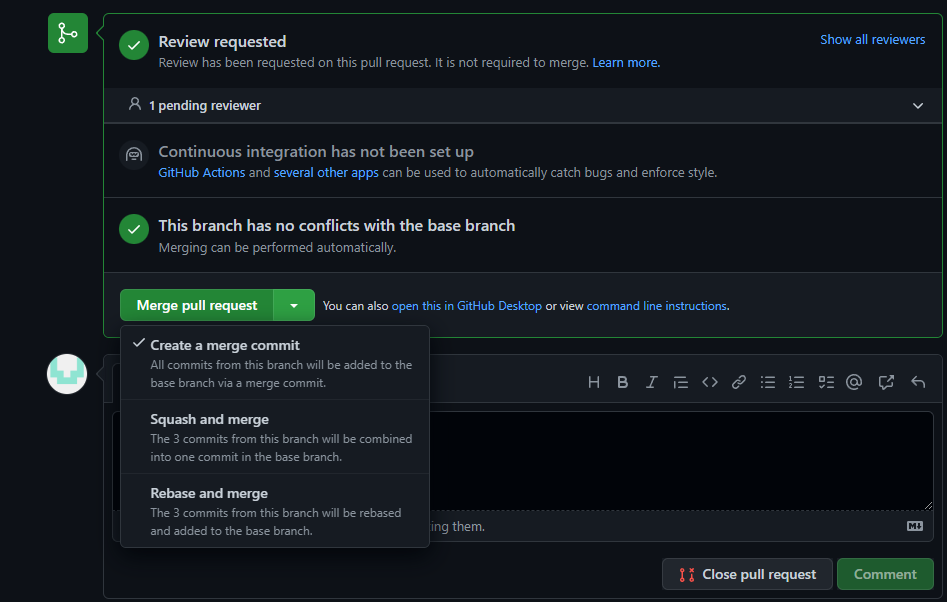
\includegraphics[width=15cm]{img/git_pull_request.png}
		\caption{Merge\textsubscript{G} di una pull request su Github\textsubscript{G}}
		La descrizione è a titolo esemplificativo, il contenuto non influenza gli smart commit\textsubscript{G} di JIRA\textsubscript{G}, il \textbf{titolo del merge\textsubscript{G} commit\textsubscript{G}} si.
		\newline 
\includegraphics[width=15cm]{img/git_pull_request_commit.png}
		\caption{Messaggio esempio per effettuare il merge\textsubscript{G} di una pull request}
	\end{figure}
	\clearpage

	\subsubsection{Issues tracking}
	JIRA\textsubscript{G}, piattaforma che offre un servizio di \textit{Issue\textsubscript{G} Tracking} è il supporto scelto vista la qualità ed il numero di servizi ed estensioni che offre.
	\newline
	La definizione dei ticket è regolata dalla seguente convenzione:
	\begin{itemize}
		\item Titolo e descrizione devono, oltre ad essere sempre presenti, esplicitare in maniera chiara il problema;
		\item Utilizzo di label;
		\item Stima del lavoro necessario al completamento;
		\item Corretto utilizzo di ereditarietà (rapporti di parentela).
	\end{itemize}
	Si è deciso di adottare il \textit{framework Scrum\textsubscript{G}} per la gestione del ciclo di sviluppo del progetto con le seguenti caratteristiche:
	\begin{itemize}
		\item Sprint\textsubscript{G} della durata di una settimana;
		\item Utilizzo di una board avente 4 stati.
		I quali sono:
		\begin{itemize}
			\item To do;
			\item In progress;
			\item In review (ogni ticket deve essere validato da uno o più componenti del gruppo per essere considerato chiuso);
			\item Done.
		\end{itemize}
	\end{itemize}

	JIRA\textsubscript{G} dispone di un'integrazione con github\textsubscript{G} che fornisce un meccanismo chiamato \textit{smart commit\textsubscript{G}} il quale permette la transizione dei ticket da uno stato ad un'altro attraverso comandi posti nei commit\textsubscript{G} stessi, la sintassi utilizzata è la seguente
	\begin{lstlisting}
	CEA-number #command <message body describing the commit\textsubscript{G}>
	\end{lstlisting}
	Tra i comandi troviamo:
	\begin{itemize}
		\item \textbf{Open}: permette di spostarsi da una issue\textsubscript{G} nello stadio "to do" oppure "in review" allo stadio "in progress";
		\item \textbf{Review}: permette lo spostamento della issue\textsubscript{G} dallo stadio "in progress" oppure "done" allo stadio "in review";
		\item \textbf{Close}: premette di spostarsi dallo stadio "in review" allo stadio "done";
		\item \textbf{Close-no-rev}: permette in casi eccezionali di passare direttamente dallo stadio "in progress" allo stadio "done".
	\end{itemize}